\documentclass[a4paper]{article}

\usepackage{amsmath}
\usepackage{graphicx}
\usepackage{hyperref}
\usepackage{subcaption} % subfigure
\usepackage{url}
%\usepackage{enumitem} % description
\usepackage{listings} % lstlisting
\usepackage{xcolor} % definecolor

% Paket für die deutsche Sprache
\usepackage[english]{babel}
%\usepackage[utf8]{inputenc}



\graphicspath{{figures/}}


%%%%%%%%%%%%%%%% C++ listings %%%%%%%%%%%%%%%%%%%%%%%%%%%%%%%%%%%
\definecolor{listinggray}{gray}{0.9}
\definecolor{lbcolor}{rgb}{0.9, 0.9, 0.9}
\definecolor{darkgreen}{rgb}{0.0, 0.2, 0.13}

\lstset{
	backgroundcolor=\color{lbcolor},
    tabsize=4,    
%   rulecolor=,
    language=[GNU]C++,
    basicstyle=\scriptsize,
    upquote=true,
    aboveskip={1.5\baselineskip},
    columns=fixed,
    showstringspaces=false,
    extendedchars=false,
    breaklines=true,
    prebreak = \raisebox{0ex}[0ex][0ex]{\ensuremath{\hookleftarrow}},
    frame=single,
    numbers=left,
    showtabs=false,
    showspaces=false,
    showstringspaces=false,
    identifierstyle=\ttfamily,
    keywordstyle=\color[rgb]{0,0,1},
	commentstyle=\color[rgb]{0.026,0.112,0.095},
	stringstyle=\color[rgb]{0.627,0.126,0.941},
	numberstyle=\color[rgb]{0.205, 0.142, 0.73},
	float,
%	\lstdefinestyle{C++}{language=C++,style=numbers}’.
}
\lstset{
	backgroundcolor=\color{lbcolor},
	tabsize=4,
	language=C++,
	captionpos=b,
	tabsize=3,
  	frame=lines,
  	numbers=left,
  	numberstyle=\tiny,
  	numbersep=5pt,
  	breaklines=true,
  	showstringspaces=false,
  	basicstyle=\footnotesize\ttfamily,
%  	identifierstyle=\color{magenta},
  	keywordstyle=\color[rgb]{0,0,1},
  	commentstyle=\color{darkgreen},
  	stringstyle=\color{red},
  	float,
  	morecomment=[l] [\color{blue}]{\#pragma}, % whole line blue if it starts with #pragma
%	morecomment=[l][\nullfont]{\%\%} % hide line if it starts with %%
}
%%%%%%%%%%%%%%%%%%%%%%%%%%%%%%%%%%%%%%%%%%%%%%%%%%%%%%%%%%%%%%%



\title{ADI for Reaction-Diffusion Systems}
\author{Stephanie Christ}
\date{August 4, 2015}

\begin{document}

\maketitle


\section{Gray-Scott Reaction-Diffusion System}

Reaction-Diffusion systems describe how the concentration of chemical substances changes in space.
The interaction of the two chemical species $U$ and $V$ is through chemical reactions, the distribution in space due to diffusion.
The reaction between the two species can be described by the following chemical terms:
\begin{align*}
	U + 2V &\rightarrow 3V \\
	V &\rightarrow P
\end{align*}
By combining the reaction and the diffusion, we obtain differential equations for the concentrations $u$ and $v$.

\begin{align}
	\frac{\partial u}{\partial t} &= D_u \Delta u - uv^2 + F(1-u) \label{eq:pde-u}\\
	\frac{\partial v}{\partial t} &= D_v \Delta v + uv^2 - (F+k)v	 \label{eq:pde-v}
\end{align}

$D_u$ and $D_v$ denote the diffusion coefficients for $u$ and $v$ respectively.
$F$ and $k$ are constant coefficient which describe at which rate the chemical reactions occur.

The model is in 2 dimensions.



\section{Numerical Method}

We split our two-dimensional domain in square cells.

To solve the equations for $u$ and $v$ (equations \ref{eq:pde-u} and \ref{eq:pde-v}), we split the reaction and the diffusion parts to solve them separately.
First, we solve the diffusion and then we add the reaction to the obtained result.
$u$ and $v$ can both be computed separately in each time step, as their contributions to the other equation is only explicit.


\subsection{Alternating Direction Implicit (ADI) method}

To solve the diffusion equation $\frac{\partial \rho}{\partial t} = D_\rho \Delta \rho$, we use the ADI method.
This method has first been proposed by Craig and Sneyd in 1988 \cite{Craig_Sneyd_1988}.

First half-step:
\begin{equation}
	\rho_{i,j}^{n+\frac{1}{2}} = \rho_{i,j}^n + \frac{D_\rho \delta t}{2} \left[ \frac{\partial^2 \rho_{i,j}^{n+\frac{1}{2}}}{\partial x^2} + \frac{\partial^2 \rho_{i,j}^n}{\partial y^2} \right]
	\label{eq:adi-half1}
\end{equation}
Second half-step:
\begin{equation}
	\rho_{i,j}^{n+1} = \rho_{i,j}^{n+\frac{1}{2}} + \frac{D_\rho \delta t}{2} \left[ \frac{\partial^2 \rho_{i,j}^{n+\frac{1}{2}}}{\partial x^2} + \frac{\partial^2 \rho_{i,j}^{n+1}}{\partial y^2} \right]
	\label{eq:adi-half2}
\end{equation}
We approximate the second derivative using a second order central differences scheme:
\begin{align}
	\frac{\partial \rho_{i,j}}{\partial x^2} &= \frac{\rho_{i-1,j} - 2 \rho_{i,j} + \rho_{i+1,j}}{\Delta x^2} \\
	\frac{\partial \rho_{i,j}}{\partial y^2} &= \frac{\rho_{i,j-1} - 2 \rho_{i,j} + \rho_{i,j+1}}{\Delta y^2}
\end{align}
Inserting this into equation \ref{eq:adi-half1} for the first half-step and setting $\Delta x = \Delta y$, we obtain the following equation:
\begin{equation}
	\rho_{i,j}^{n+\frac{1}{2}} = \rho_{i,j}^n + \frac{D_\rho \delta t}{2} \left[ \frac{\rho_{i-1,j}^{n+\frac{1}{2}} - 2 \rho_{i,j}^{n+\frac{1}{2}} + \rho_{i+1,j}^{n+\frac{1}{2}}}{\Delta x^2} + \frac{\rho_{i-1,j}^n - 2 \rho_{i,j}^n + \rho_{i+1,j}^n}{\Delta x^2} \right]
\end{equation}
We sort the implicit and explicit parts and get the following system:
\begin{multline}
	-\frac{D_\rho \Delta t}{2 \Delta x^2} \rho_{i-1,j}^{n + \frac{1}{2}} + \left( 1 + \frac{D_\rho \Delta t}{\Delta x^2} \right) \rho_{i,j}^{n + \frac{1}{2}} - \frac{D_\rho \Delta t}{2 \Delta x^2} \rho_{i+1,j}^{n + \frac{1}{2}} \\
	= \frac{D_\rho \Delta t}{2 \Delta x^2} \rho_{i,j-1}^n + \left( 1 - \frac{D_\rho \Delta t}{\Delta x^2} \right) \rho_{i,j}^n - \frac{D_\rho \Delta t}{2 \Delta x^2} \rho_{i,j+1}^n
\end{multline}
This gives us a tridiagonal system with a constant on each diagonal for each row of the domain.
On the lower and upper diagonals, we have the coefficient $-\frac{D_\rho \Delta t}{2 \Delta x^2}$, on the middle diagonal the coefficient $\left( 1 + \frac{D_\rho \Delta t}{\Delta x^2} \right)$.

Performing analogous calculations for the second half-step \ref{eq:adi-half2} yields
\begin{multline}
	-\frac{D_\rho \Delta t}{2 \Delta x^2} \rho_{i,j-1}^{n + 1} + \left( 1 + \frac{D_\rho \Delta t}{\Delta x^2} \right) \rho_{i,j}^{n + 1} - \frac{D_\rho \Delta t}{2 \Delta x^2} \rho_{i,j+1}^{n + 1} \\
	= \frac{D_\rho \Delta t}{2 \Delta x^2} \rho_{i-1,j}^{n + \frac{1}{2}} + \left( 1 - \frac{D_\rho \Delta t}{\Delta x^2} \right) \rho_{i,j}^{n + \frac{1}{2}} - \frac{D_\rho \Delta t}{2 \Delta x^2} \rho_{i+1,j}^{n + \frac{1}{2}}
\end{multline}
The second half-step gives a tridiagonal system to solve for each column of the domain.

\subsubsection{Thomas Algorithm}
The Thomas Algorithm -- named after Llewellyn Thomas -- is an algorithm to solve tridiagonal systems $Ax = d$ in $\mathcal O(n)$ time.
It is a form of Gaussian Elimination.
\begin{align}
	Ax &= d \\
\begin{bmatrix}
   {b_0} & {c_0} & {   } & {   } & { 0 } \\
   {a_1} & {b_1} & {c_1} & {   } & {   } \\
   {   } & {a_2} & {b_2} & \ddots & {   } \\
   {   } & {   } & \ddots & \ddots & {c_{n-1}}\\
   { 0 } & {   } & {   } & {a_n} & {b_n}\\
\end{bmatrix}
\begin{bmatrix}
   {x_0 }  \\
   {x_1 }  \\
   {x_2 }  \\
   \vdots   \\
   {x_n }  \\
\end{bmatrix}
&=
\begin{bmatrix}
   {d_0 }  \\
   {d_1 }  \\
   {d_2 }  \\
   \vdots   \\
   {d_n }  \\
\end{bmatrix}
\end{align}
The method first modifies the coefficients in the following way:
\begin{align}
	c'_i &=
\begin{cases}
\begin{array}{lcl}
  \cfrac{c_i}{b_i}                  & ; & i = 0 \\
  \cfrac{c_i}{b_i - a_i c'_{i - 1}} & ; & i = 1, 2, \dots, n-1 \\
\end{array}
\end{cases} \\
d'_i &=
\begin{cases}
\begin{array}{lcl}
  \cfrac{d_i}{b_i}                  & ; & i = 0 \\
  \cfrac{d_i - a_i d'_{i - 1}}{b_i - a_i c'_{i - 1}} & ; & i = 1, 2 \dots, n. \\
\end{array}
\end{cases}
\end{align}
Then the solution is obtained by backwards substitution.
\begin{align}
	x_n &= d'_n \\
	x_i &= d'_i - c'_i x_{i + 1} \qquad ; \ i = n - 1, n - 2, \ldots, 0.
\end{align}


\subsection{Reaction Term}
To add the reaction term to the solution of the diffusion equation, we use a forward Euler scheme.
$\tilde u^{n+1}$ and $\tilde v^{n+1}$ denote the solution of the diffusion equations before adding the contribution of the reaction term.

\begin{align}
	u_{i,j}^{n+1} &= \tilde u_{i,j}^{n+1} + \Delta t \left( - \tilde u_{i,j}^{n+1} (\tilde v_{i,j}^{n+1})^2 + F ( 1- \tilde u_{i,j}^{n+1} ) \right) \\
	v_{i,j}^{n+1} &= \tilde v_{i,j}^{n+1} + \Delta t \left( \tilde u_{i,j}^{n+1} (\tilde v_{i,j}^{n+1})^2 - (F+k) \tilde v_{i,j}^{n+1} \right)
\end{align}


\subsection{Boundary conditions}
We use reflecting boundary conditions.
This modifies the tridiagonal matrix system, so that the values on each diagonal aren't constant for the whole diagonal anymore.
The first value on the upper diagonal, as well as the last value on the lower diagonal, are doubled.



\section{Implementation}

We save the grid for $u$ and $v$ each in a \verb+std::vector<double>+ in row-wise storage.
For the tridiagonal matrix, we wrote our own class to simplify the access to the diagonals.

To visualize the result, we used OpenGL for displaying the concentration of $u$ during the computation, and LodePNG\footnote{http://lodev.org/lodepng/} -- a PNG image encoder and decoder by Lode Vandevenne -- to save the image after the simulation.

\subsection{Serial version}

We loop over all time steps and apply the numerical scheme described above.

%«noindent\begin{minipage}{\linewidth}
%\begin{lstlisting}[label={lst:loop-time}, caption={Loop over all time steps}]
%for (int i=0; i<nSteps_; ++i) {
%	step();
%}
%\end{lstlisting}
%\end{minipage}


In each step, we first apply the ADI method to $u$ and $v$ to solve the diffusion part of the problem.
Then we solve the reaction.

For the ADI-step, we have to treat the boundary rows/columns differently, as the dependencies on the neighbouring cells change (see \ref{lst:adi-serial}.
To facilitate the access to a grid cell, we have defined macros that let us use the two-dimensional coordinates of the cells.
The solver for the tridiagonal matrix is an implementation of the Thomas algorithm, see section \ref{sec:thomas}.


\begin{lstlisting}[label={lst:adi-serial}, caption={Serial implementation of the first half-step (the computations for $v$ are omitted as they are analogue to the computation for $u$)}, float]
// loop over all rows

// j=0
for (int i=0; i<N_; ++i) {
    uRhs[i] = U(i,0) + uCoeff * (U(i,1) - U(i,0));
}
TriDiagMatrixSolver::solve(N_, matU1_, uRhs, &UHALF(0,0), 1);

// inner grid points
for (int j=1; j<N_-1; ++j) {
    // create right-hand side of the systems
    for (int i=0; i<N_; ++i) {
        uRhs[i] = U(i,j) + uCoeff * (U(i,j+1) - 2.*U(i,j) + U(i, j-1));
    }
    
    TriDiagMatrixSolver::solve(N_, matU1_, uRhs, &UHALF(0,j), 1);
}

// j=N_-1
for (int i=0; i<N_; ++i) {
    uRhs[i] = U(i,N_-1) + uCoeff * (- U(i,N_-1) + U(i,N_-2));
}
TriDiagMatrixSolver::solve(N_, matU1_, uRhs, &UHALF(0,N_-1), 1);
\end{lstlisting}

The second half-step is implemented analogously to the first half-step, but with the outermost loop over the columns \verb+i+ instead of the rows \verb+j+.

For the reaction, we used a simple loop over all grid cells and add the reaction term to $u$ and $v$ (see listing \ref{lst:reaction}).

\begin{lstlisting}[label={lst:reaction}, caption={Reaction, serial implementaion}]
double tmp;
for (int i=0; i<N_; ++i) {
    for (int j=0; j<N_; ++j) {
        tmp = U(i,j);
        U(i,j) += dt_ * ( -tmp*V(i,j)*V(i,j) + F_*(1.-tmp) );
        V(i,j) += dt_ * ( tmp*V(i,j)*V(i,j) - (F_+k_)*V(i,j) );
    }
}
\end{lstlisting}



\subsection{Thomas Algorithm}\label{sec:thomas}
For the implementation of the Thomas Algorithm, we used the version on wikipedia from April 2014 \cite{wiki:thomas-alg}.
We modified it so that we can pass the whole grid as an argument.
Since the access to the grid is row-/column-wise, the argument \verb+result+ is a pointer to the first element we want to access.
The increment \verb+inc+ is the increment we need to access the next element in the result.
It is different for row-wise and column-wise access (e.g. first or second half-step), either $1$ or $N$ (the size of the grid in one dimension).

\begin{lstlisting}[label={lst:thomas-dec}, caption={Declaration of our implementation of the Thomas algorithm}, float]
namespace TriDiagMatrixSolver
{
    /**
     * Solve a tridiagonal matrix system.
     * 
     * @param n         number of elements in the result
     * @param mat       tridiagonal matrix
     * @param rhs       right-hand side of the system
     * @param result    vector for the result, pointer to the first element
     * @param inc       increment for the elements of the result
     */
    void solve(unsigned int n, const TriDiagMatrix& mat, const std::vector<double>& rhs, double *result, const unsigned int inc);
};
\end{lstlisting}


\subsection{Parallelization}

\subsubsection{OpenMP}
First, we parallelized our code using OpenMP.
In the diffusion part, we parallelized the outer \verb+for+-loop (over \verb+j+ in the listing \ref{lst:adi-serial}), since there are only read-dependencies between different \verb+j+.
The parallelization is according to listing \ref{lst:adi-omp}.

\begin{lstlisting}[label={lst:adi-omp}, caption={Parallel OpenMP region}, float]
#pragma omp parallel num_threads(nthreads_)
{ // PARALLEL REGION BEGIN

// right hand sides for u and for v
std::vector<double> puRhs(N_);
std::vector<double> pvRhs(N_);

#pragma omp for
for (int j=1; j<N_-1; ++j) {
    // row-wise computations, see listing 1
}

} // PARALLEL REGION END
\end{lstlisting}
The boundary computations aren't parallelized.
We do not need to declare anything private, because each thread declares its own right-hand side, and all other variables have either read-only access or are accessed in different regions by each thread.

In the reaction part, we also parallelized the outer loop with a \\
\verb+#pragma omp parallel for+

\subsubsection{MPI}
\paragraph{Domain decomposition}
For the MPI version, we decompose the domain and distribute it between the processes.
This was done in blocks of rows, see figure \ref{fig:domain-decomp}.
To be able to distribute the rows equally, we changed the size of the domain to a multiple of the number of processors.
As the first and last row need to access the values from the rows above/below, we add ghost rows (see figure \ref{fig:domain-decomp-ghost}).
The ghost rows don't get written to, but read, and need to be exchanged between processes before the computations.
The grid is initialized on the different processes, so that each process has a vector of size $N \times (N_{loc}+2)$ for its part of the grid.
The first and last row are for the ghost cells, so the processes only initialize $N \times N_{loc}$ elements.

\begin{figure}
	\centering
	\begin{subfigure}{0.45\textwidth}
		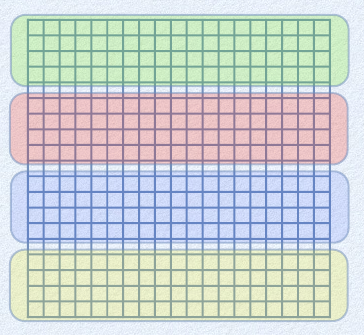
\includegraphics[height=\textwidth]{domain_decomposition.png}
		\caption{Domain decomposition}
		\label{fig:domain-decomp}
	\end{subfigure}
	\quad
	\begin{subfigure}{0.45\textwidth}
		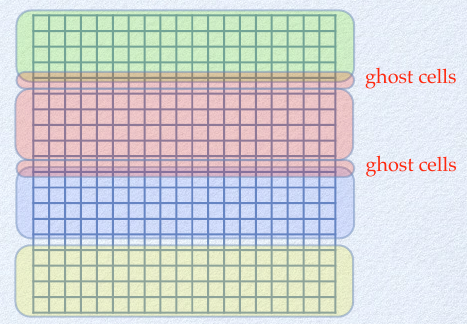
\includegraphics[height=\textwidth]{ghostcells.png}
		\caption{Ghost cells (for red)}
		\label{fig:domain-decomp-ghost}
	\end{subfigure}
	\caption{Domain decomposition for 4 MPI processes\protect\footnotemark}
	\label{fig:domain-decomp-mpi}
\end{figure}

\footnotetext{Figures from HPCSE slides}

\begin{lstlisting}[label={lst:mpi-communication}, caption={Communication of the ghost cells}, float]
MPI_Request request[8];
MPI_Status status[8];

// exchange boundaries
if (world.coord_x % 2 == 0) {
    
    MPI_Isend(&u_[(Nx_loc)*(Ny_loc)],   1, bottom_boundary, world.bottom_proc, TAG, cart_comm, &request[0]);
    MPI_Irecv(&u_[(Nx_loc+1)*(Ny_loc)], 1, bottom_boundary, world.bottom_proc, TAG, cart_comm, &request[1]);
    MPI_Isend(&u_[(Ny_loc)],            1, top_boundary,    world.top_proc,    TAG, cart_comm, &request[2]);
    MPI_Irecv(&u_[0],                   1, top_boundary,    world.top_proc,    TAG, cart_comm, &request[3]);
}
else {
    
    MPI_Irecv(&u_[0],                   1, top_boundary,    world.top_proc,    TAG, cart_comm, &request[0]);
    MPI_Isend(&u_[(Ny_loc)],            1, top_boundary,    world.top_proc,    TAG, cart_comm, &request[1]);
    MPI_Irecv(&u_[(Nx_loc+1)*(Ny_loc)], 1, bottom_boundary, world.bottom_proc, TAG, cart_comm, &request[2]);
    MPI_Isend(&u_[(Nx_loc)*(Ny_loc)],   1, bottom_boundary, world.bottom_proc, TAG, cart_comm, &request[3]);

}
\end{lstlisting}

\begin{lstlisting}[label={lst:adi-mpi}, caption={First half-step parallelized with MPI}, float]
// send/receive ghost cells (non-blocking)

// update inner grid points (see listing 1)

// wait for boundaries to arrive
MPI_Waitall(8,request,status);


// update local boundaries

if (world.rank == 0) {
    // i=0 local and global
    for (int j=0; j<N_; ++j) {
        uRhs[j] = U(0,j) + uCoeff * (U(1,j) - U(0,j));
    }
    TriDiagMatrixSolver::solve(N_, matU1_, uRhs, &UTEMP(0,0), 1);
}
else {
    // i=0 local
    for (int j=0; j<N_; ++j) {
        uRhs[j] = U(0,j) + uCoeff * (U(0+1,j) - 2.*U(0,j) + U(0-1,j));
    }
    TriDiagMatrixSolver::solve(N_, matU1_, uRhs, &UTEMP(0,0), 1);
}


if (world.rank == world.size-1) {
    // i=Nx_loc-1 local and i=N_-1 global
    for (int j=0; j<N_; ++j) {
        uRhs[j] = U(Nx_loc-1,j) + uCoeff * (- U(Nx_loc-1,j) + U(Nx_loc-2,j));
    }
    TriDiagMatrixSolver::solve(N_, matU1_, uRhs, &UTEMP(Nx_loc-1,0), 1);
}
else {
    // i=Nx_loc-1 local
    for (int j=0; j<N_; ++j) {
        uRhs[j] = U(Nx_loc-1,j) + uCoeff * (U(Nx_loc-1+1,j) - 2.*U(Nx_loc-1,j) + U(Nx_loc-1-1,j));
    }
    TriDiagMatrixSolver::solve(N_, matU1_, uRhs, &UTEMP(Nx_loc-1,0), 1);
}
\end{lstlisting}

\paragraph{Communication}
The ghost cells are sent/received by the processes as shown in listing \ref{lst:mpi-communication}.
We used nonblocking communication, because that lets us update the local inner grid cells (independent of ghost cells), while we wait on the ghost cells to arrive.
After updating the inner grid cells, we need to wait for the boundaries to arrive, then we can continue to update the boundary cells.
We distinguish between rows that are only local boundaries, and those that are also global boundaries (first and last row), because they need to handle the reflecting boundary conditions correctly.

\paragraph{Transposing the grid}
After the first half-step, we need to transpose the grid, so that instead of the columns like in the serial version, we can work again on rows that are distributed between processes.
For the transposing, we have implemented two different versions.
Both versions first split the rows into blocks, such that each processor has a row of blocks.
See figure \ref{fig:domain-decomp-block} for a visualization of the blocks (all colours are split into blocks analogue to the green blocks that are shown).
\begin{figure}
	\centering
	\begin{subfigure}{0.45\textwidth}
		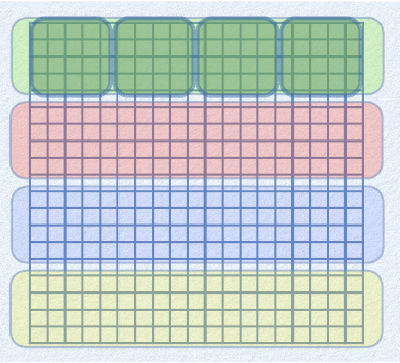
\includegraphics[width=\textwidth]{domain_decomposition_transpose.png}
		\caption{First row of blocks before transposing}
		\label{fig:domain-decomp-block-before}
	\end{subfigure}
	\quad
	\begin{subfigure}{0.45\textwidth}
		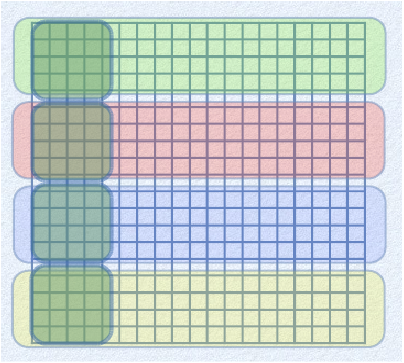
\includegraphics[width=\textwidth]{domain_decomposition_transpose_after.png}
		\caption{First row (now column) of blocks after transposing}
		\label{fig:domain-decomp-block-after}
	\end{subfigure}
	\caption{Domain decomposition for MPI transpose\protect\footnotemark}
	\label{fig:domain-decomp-block}
\end{figure}
\footnotetext{Figures adapted from HPCSE slides}
The processes send the blocks to another process using \verb+MPI_Alltoall+.
The first version then transposes each block locally (see listing \ref{lst:mpi-transpose-local}).
The second version uses a different receive data type than send data type.
The receiving data type is ordered in a way that is the transpose of the send data type (see listing \ref{lst:mpi-transpose-datatype}).
This lets us skip the local transpose, as the received data is already transposed.
We compare the performance of these two versions in section \ref{sec:time-serial-transpose}.

\begin{lstlisting}[label={lst:mpi-transpose-local}, caption={Transposing the grid using MPI Alltoall and local transpose}, float]
MPI_Alltoall(&uTemp[Ny_loc], 1, block_resized_send, &u_[Ny_loc], 1, block_resized_send, MPI_COMM_WORLD);
        
// locally transpose blocks
int ind1, ind2;
// loop over blocks
for (int b=0; b<Nb_loc; ++b) {
    for (int i=0; i<Nx_loc; ++i) {
        for (int j=0; j<i; ++j) {
            ind1 = (i+1)*Ny_loc + j + b*Nx_loc; // regular index + offset of block
            ind2 = (j+1)*Ny_loc + i + b*Nx_loc; // switch i and j
                    
            std::swap(u_[ind1], u_[ind2]);
        }
    }
}
\end{lstlisting}
\begin{lstlisting}[label={lst:mpi-transpose-datatype}, caption={Transposing the grid using MPI Alltoall and different send/receive datatypes}, float]
MPI_Alltoall(&uTemp[Ny_loc], 1, block_resized_send, &u_[Ny_loc], 1, block_resized_recv, MPI_COMM_WORLD);
\end{lstlisting}

After transposing the grid, the second half-step is identical to the first half-step.

The reaction part of the simulation isn't changed from the serial implementation, except that the loop goes only over the local grid.

\paragraph{MPI Data types}
We defined four different MPI data types.
Two are for the ghost cells (top and bottom rows), they are both identical and only defined twice for code readability (see listing \ref{lst:datatypes-ghost}).
These data types are contiguous vectors.
The other two are to transpose the grid (see listing \ref{lst:datatypes-transpose}).
They are square blocks that split the blocks of rows each processor has.
\verb+block_send+ and \verb+block_recv+ already contain the data we need to send/receive in the correct form, however for \verb+MPI_Alltoall+ the data needs to be contiguous, which we achieve with \verb+MPI_Type_create_resized+.

%\noindent\begin{minipage}{\linewidth} % prevents page break in listing
\begin{lstlisting}[label={lst:datatypes-ghost}, caption={MPI data types for ghost cells}, float]
// build contiguous (rows) vectors for boundaries
MPI_Type_contiguous(Ny_loc, MPI_DOUBLE, &bottom_boundary);
MPI_Type_commit(&bottom_boundary);

MPI_Type_contiguous(Ny_loc, MPI_DOUBLE, &top_boundary);
MPI_Type_commit(&top_boundary);
\end{lstlisting}
%\end{minipage}


\begin{lstlisting}[label={lst:datatypes-transpose}, caption={MPI data types for transposing the grid}, float]
MPI_Datatype block_send, block_col, block_recv;


// send data type
int sizes[2]    = {Nx_loc, Ny_loc}; // size of global array
int subsizes[2] = {Nx_loc, Nx_loc}; // size of sub-region
int starts[2]   = {0,0}; // where does the first subarray begin

MPI_Type_create_subarray(2, sizes, subsizes, starts, MPI_ORDER_C, MPI_DOUBLE, &block_send);
MPI_Type_commit(&block_send);

// resize -> make contiguous
MPI_Type_create_resized(block_send, 0, Nx_loc*sizeof(double), &block_resized_send);
MPI_Type_free(&block_send);
MPI_Type_commit(&block_resized_send);


// receive data type (only used when not transposing locally)
// create one row of the block
MPI_Type_vector(Nx_loc, 1, Ny_loc, MPI_DOUBLE, &block_col);
MPI_Type_commit(&block_col);
// combine rows into block
MPI_Type_hvector(Nx_loc, 1, sizeof(double), block_col, &block_recv);
MPI_Type_free(&block_col);
MPI_Type_commit(&block_recv);

// resize -> make contiguous
MPI_Type_create_resized(block_recv, 0, sizeof(double), &block_resized_recv);
MPI_Type_free(&block_recv);
MPI_Type_commit(&block_resized_recv);
\end{lstlisting}



\subsubsection{Hybrid OpenMP + MPI}
The hybrid version of the algorithm is very close to the MPI version.
We parallelized the update of the inner grid cells as we did in the pure OpenMP version.
We also added a \verb+#pragma omp parallel for+ clause to the local transposing of the blocks (if applicable) and the reaction part of the simulation.


\section{Results}

\subsection{Patterns}
We compared our resulting patterns with the patterns Pearson showed in his paper \cite{pearson_1993}.
Most patterns are close to the ones Pearson got, the pattern $\iota$ differs most.
However, these differences are likely due to having slightly different parameters than Pearson, as we had to read them out of the parameter space.

\begin{figure}
	\centering
	\captionsetup{format=hang}
	\begin{subfigure}{0.2\textwidth}
		\includegraphics[width=\textwidth]{patterns/{alpha_k_0.046_F_0.007_step_100000}.png}
		\caption{Pattern $\alpha$\\$F=0.007$\\$k=0.046$}
		\label{fig:pattern-alpha}
	\end{subfigure}
	\quad
	\begin{subfigure}{0.2\textwidth}
		\includegraphics[width=\textwidth]{patterns/{beta_k_0.046_F_0.020_step_100000}.png}
		\caption{Pattern $\beta$\\$F=0.020$\\$k=0.046$}
		\label{fig:pattern-beta}
	\end{subfigure}
	\quad
	\begin{subfigure}{0.2\textwidth}
		\includegraphics[width=\textwidth]{patterns/{gamma_k_0.055_F_0.024_step_100000}.png}
		\caption{Pattern $\gamma$\\$F=0.024$\\$k=0.055$}
		\label{fig:pattern-gamma}
	\end{subfigure}
	\quad
	\begin{subfigure}{0.2\textwidth}
		\includegraphics[width=\textwidth]{patterns/{delta_k_0.055_F_0.030_step_100000}.png}
		\caption{Pattern $\delta$\\$F=0.030$\\$k=0.055$}
		\label{fig:pattern-delta}
	\end{subfigure}
	
	\begin{subfigure}{0.2\textwidth}
		\includegraphics[width=\textwidth]{patterns/{epsilon_k_0.055_F_0.019_step_100000}.png}
		\caption{Pattern $\epsilon$\\$F=0.019$\\$k=0.055$}
		\label{fig:pattern-epsilon}
	\end{subfigure}
	\quad
	\begin{subfigure}{0.2\textwidth}
		\includegraphics[width=\textwidth]{patterns/{xi_k_0.061_F_0.024_step_100000}.png}
		\caption{Pattern $\zeta$\\$F=0.024$\\$k=0.061$}
		\label{fig:pattern-zeta}
	\end{subfigure}
	\quad
	\begin{subfigure}{0.2\textwidth}
		\includegraphics[width=\textwidth]{patterns/{eta_k_0.063_F_0.035_step_100000}.png}
		\caption{Pattern $\eta$\\$F=0.035$\\$k=0.063$}
		\label{fig:pattern-eta}
	\end{subfigure}
	\quad
	\begin{subfigure}{0.2\textwidth}
		\includegraphics[width=\textwidth]{patterns/{theta_k_0.060_F_0.042_step_100000}.png}
		\caption{Pattern $\theta$\\$F=0.042$\\$k=0.060$}
		\label{fig:pattern-theta}
	\end{subfigure}
	
	\begin{subfigure}{0.2\textwidth}
		\includegraphics[width=\textwidth]{patterns/{iota_k_0.060_F_0.050_step_100000}.png}
		\caption{Pattern $\iota$\\$F=0.050$\\$k=0.060$}
		\label{fig:pattern-iota}
	\end{subfigure}
	\quad
	\begin{subfigure}{0.2\textwidth}
		\includegraphics[width=\textwidth]{patterns/{kappa_k_0.063_F_0.050_step_100000}.png}
		\caption{Pattern $\kappa$\\$F=0.050$\\$k=0.063$}
		\label{fig:pattern-kappa}
	\end{subfigure}
	\quad
	\begin{subfigure}{0.2\textwidth}
		\includegraphics[width=\textwidth]{patterns/{lambda_k_0.065_F_0.040_step_100000}.png}
		\caption{Pattern $\lambda$\\$F=0.040$\\$k=0.065$}
		\label{fig:pattern-lambda}
	\end{subfigure}
	\quad
	\begin{subfigure}{0.2\textwidth}
		\includegraphics[width=\textwidth]{patterns/{mu_k_0.065_F_0.050_step_100000}.png}
		\caption{Pattern $\mu$\\$F=0.050$\\$k=0.065$}
		\label{fig:pattern-mu}
	\end{subfigure}
	\caption{Patterns after $10^5$ steps}
	\label{fig:patterns}
\end{figure}


\subsection{Serial version}
For the serial version, we ran it with and without compiler vectorization.
With vectorization, we compiled using \verb|g++ -ftree-vectorize ...|, without we used \verb|g++ -fno-tree-vectorize ...|.
The comparison of the system size scaling of these two version can be seen in figure \ref{fig:serial-vecnovec}.
It is clearly visible, that it doesn't make a difference whether the compiler vectorizes the code or not.
We fitted a line with python \verb|numpy.polyfit| and obtained a scaling exponent of $2.2$.

\begin{figure}
	\centering
	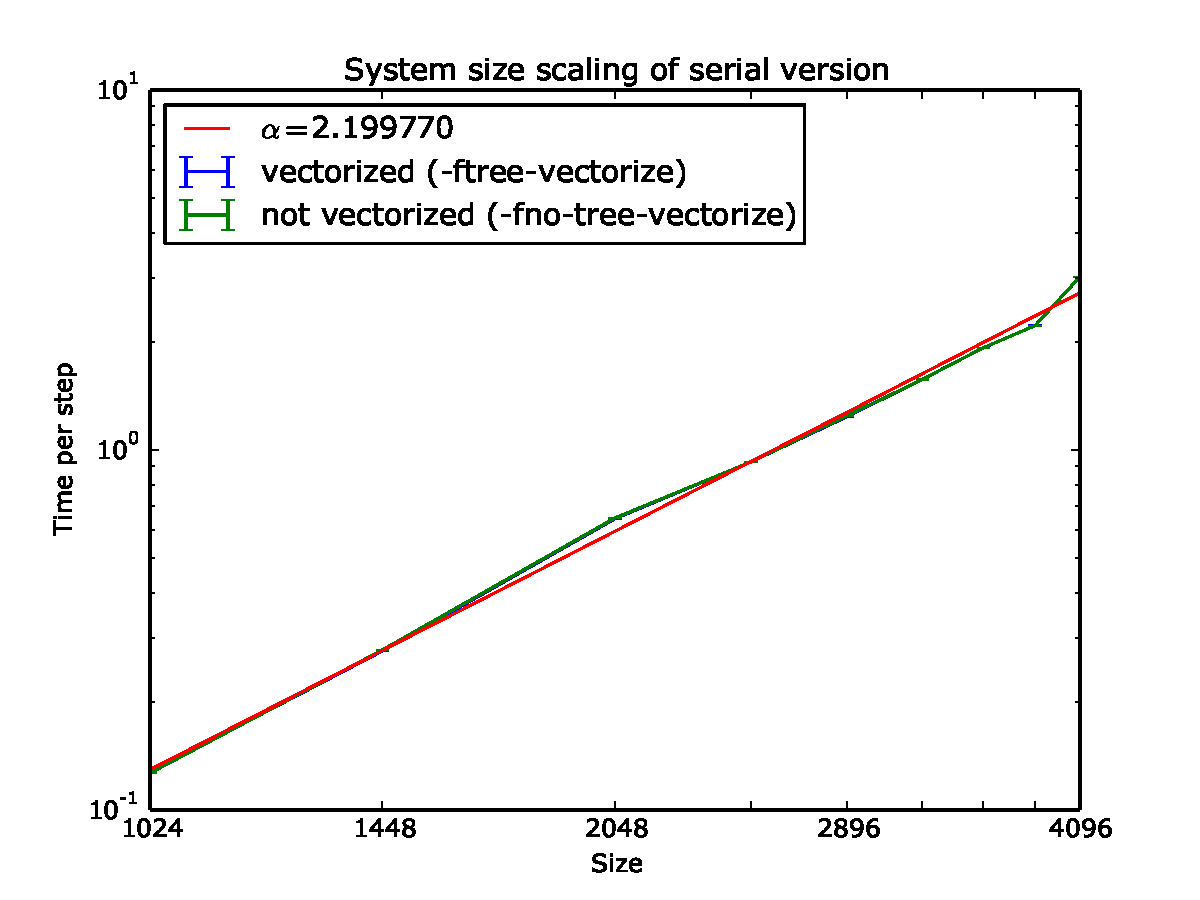
\includegraphics[width=0.9\textwidth]{serial_vecnovec_2.pdf}
	\caption{System size scaling of the serial version with and without compiler vectorization}
	\label{fig:serial-vecnovec}
\end{figure}

\subsection{OpenMP version}






\clearpage
\bibliographystyle{plain}
\bibliography{refs}


\end{document}
